%%%%%%%%%%%%%%%%%%%%%%%%%%%%%%%%%%
%% UE 1 - 03c Phonologie
%%%%%%%%%%%%%%%%%%%%%%%%%%%%%%%%%%

\begin{frame}
\frametitle{Übung -- Lösung}

\begin{minipage}{.45\textwidth}
\centering
\scalebox{.75}{	
\begin{forest} MyP edges, [,phantom
[$\sigma$
[O	[x, tier=word [\textipa{S}]
]
[x, tier=word [\textipa{p}]
]
[x, tier=word[\textipa{\textscr}]
]
]
[R
[N	[x, tier=word [\textipa{E}]
]
]
[K, name=K	[x,name=x  [\textipa{\c{c}}]
]
]
]  
]
[$\sigma$
[O, name=O]
[R
[N	[x[\textipa{@}]
]
]
[K	[x[\textipa{n}]
]
]
]
]
]
\draw[black] (O.south)--(x.north);
\end{forest}
}
\end{minipage}
\pause
%
\begin{minipage}{.05\textwidth}
\hfill
\end{minipage}
%
\begin{minipage}{.45\textwidth}
%%%%%%%%%%%%%%%
%%% Forestset Syllables

\newbox\foreststrutbox
\setbox\foreststrutbox=\hbox to 0pt{\phantom{\forestOve{standard node}{content}}}
\def\foreststrut{\copy\foreststrutbox}
\forestset{
GP1/.style 2 args={
for n={1}{baseline},
s sep=0pt, l sep=0pt,
for descendants={
l sep=0pt, l={#1},
anchor=base,calign=first,child anchor=north,
inner xsep=1pt,inner ysep=2pt,outer sep=0pt,s sep=0pt,
},
delay={
if content={}{phantom}{for children={no edge}},
for tree={
if content={O}{tier=OR}{},
if content={R}{tier=OR}{},
if content={N}{tier=N}{},
if content={x}{
tier=x,content={$\times$},outer xsep={#2},
for tree={calign=center},
for descendants={content format={\foreststrut\forestoption{content}}},
before drawing tree={outer xsep=0pt,delay={typeset node}},
s sep=4pt
}{},
},
},
before drawing tree={where content={}{parent anchor=center,child anchor=center}{}},
},
GP1/.default={5ex}{8.0pt},
associate/.style={%
tikz+={\draw(!)--(!#1);}},
spread/.style={
before drawing tree={tikz+={\draw[dotted](!)--(!#1);}}},
govern/.style={
before drawing tree={tikz+={\draw[->](!)--(!#1);}}},
p-govern/.style={
before drawing tree={tikz+={\draw[->](.north) to[out=150,in=30] (!#1.north);}}},
no p-govern/.style={
before drawing tree={tikz+={\draw[->,loosely dashed](.north) to[out=150,in=30] (!#1.north);}}},
encircle/.style={before drawing tree={circle,draw,inner sep=0pt}},
fen/.style={pin={[font=\footnotesize,inner sep=1pt,pin edge=<-]10:\textsc{Fen}}},
el/.style={content=\textsc{\textbf{##1}}},
head/.style={content=\textsc{\textbf{\underline{##1}}}},
llap/.style={
tikz+={%
\edef\forest@temp{\noexpand\node[\option{node options},
anchor=base east,at=(.base east)]}%
\forest@temp{#1\phantom{\option{environment}}};
}
},
rlap/.style={
tikz+={%
\edef\forest@temp{\noexpand\node[\option{node options},
anchor=base west,at=(.base west)]}%
\forest@temp{\phantom{\option{environment}}#1};
}
},
}
%%%%%%%%%%%%%

\centering
%\visible<3->
{\scalebox{.75}{\begin{forest} MyP edges, [,phantom
[$\sigma$
[O	[x, tier=word[\textipa{P}]
]
]
[R
[N
[x, tier=word[\textipa{o:}, name=o]
]
[x, name=x]
%    		{\draw[black] (.south)--++(-2.38em,-1.7ex);}
]
[K
[x[\textipa{p}]
]
[x[\textipa{s}]
]
[x[\textipa{t}]
]
]
]  
] ]
\draw[black](x.south)--(o.north);
\end{forest}}}
\end{minipage}
\pause
\begin{minipage}{.45\textwidth}
\begin{figure}
\centering
%		\visible<2->
{\scalebox{.75}{
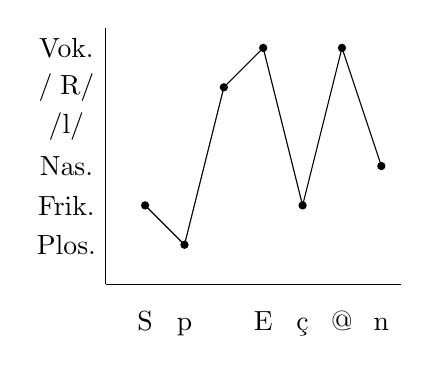
\begin{tikzpicture}[scale=0.5]
\draw[black] (-1,0) -- (6.5,0) ; % x axis
\draw[black] (-1,0) -- (-1,6.5); % y axis
\node at (-2,1) {Plos.};
\node at (-2,2) {Frik.};
\node at (-2,3) {Nas.};
\node at (-2,4) {\textipa{/l/}};
\node at (-2,5) {\textipa{/\;R/}};
\node at (-2,6) {Vok.};
\draw[black] (0,2) -- (1,1) -- (2,5) -- (3,6) -- (4,2) -- (5,6) -- (6,3);
\node at (0,-1) {\strut \textipa{S}};
\node at (1,-1) {\strut \textipa{p}};
\node at (2,-1) {\strut \textipa{\textscr}};
\node at (3,-1) {\strut \textipa{E}};
\node at (4,-1) {\strut \textipa{\c{c}}};
\node at (5,-1) {\strut \textipa{@}};
\node at (6,-1) {\strut \textipa{n}};
\fill (0,2) circle [radius=3pt];
\fill (1,1) circle [radius=3pt];
\fill (2,5) circle [radius=3pt];
\fill (3,6) circle [radius=3pt];
\fill (4,2) circle [radius=3pt];
\fill (5,6) circle [radius=3pt];
\fill (6,3) circle [radius=3pt];
\end{tikzpicture}}}
\end{figure}
\end{minipage}
\pause
\begin{minipage}{.05\textwidth}
\hfill
\end{minipage}
\begin{minipage}{.45\textwidth}
\begin{figure}
\centering
%\visible<4->
{\scalebox{.75}{
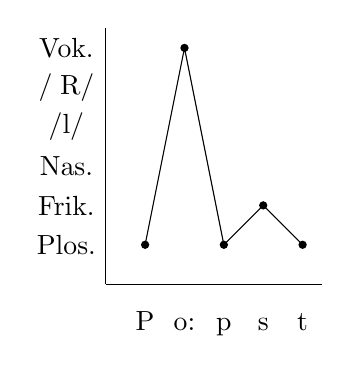
\begin{tikzpicture}[scale=0.5]
\draw[black] (-1,0) -- (4.5,0) ; % x axis
\draw[black] (-1,0) -- (-1,6.5); % y axis
\node at (-2,1) {Plos.};
\node at (-2,2) {Frik.};
\node at (-2,3) {Nas.};
\node at (-2,4) {\textipa{/l/}};
\node at (-2,5) {\textipa{/\;R/}};
\node at (-2,6) {Vok.};
\draw[black] (0,1) -- (1,6) -- (2,1) -- (3,2) -- (4,1);
\node at (0,-1) {\strut \textipa{P}};
\node at (1,-1) {\strut \textipa{o:}};
\node at (2,-1) {\strut \textipa{p}};
\node at (3,-1) {\strut \textipa{s}};
\node at (4,-1) {\strut \textipa{t}};
\fill (0,1) circle [radius=3pt];
\fill (1,6) circle [radius=3pt];
\fill (2,1) circle [radius=3pt];
\fill (3,2) circle [radius=3pt];
\fill (4,1) circle [radius=3pt];
\end{tikzpicture}}}
\end{figure}
\end{minipage}

\end{frame}
%%%%%%%%%%%%%%%%%%%%%%%%%%%%%%%%%

\begin{frame}
\frametitle{Übung -- Lösung}
%
\begin{minipage}{.3\textwidth}
\centering
\scalebox{.75}{\begin{forest} MyP edges, [,phantom
[$\sigma$
[O
[x, tier=word[\textipa{b}]]
[x, tier=word[\textipa{\textscr}]]
]
[R
[N	[x, tier=word[\textipa{a}]]
]
[K
[x[\textipa{n}]]
[x[\textipa{t}]]
]
]  
]
[$\sigma$
[O	[x, tier=word[\textipa{S}]]
]
[R	
[N	
[x[\textipa{U}]]
]
[K	
[x[\textipa{\t{ts}}]]
]
]
]]
\end{forest}}

\end{minipage}
\pause
%
\begin{minipage}{.02\textwidth}
\hfill
\end{minipage}
%
\begin{minipage}{.65\textwidth}
\centering
\scalebox{.75}{
\begin{forest}
MyP edges, [, phantom
[$ \sigma $
[O
[x, tier=word[\textipa{P}]]
]
[R
[N
[x, tier=word[\textipa{a}]]
]
[K
[x[\textipa{p}]]
]
]
]
[$ \sigma $
[O
[x, tier=word[\textipa{S}]]
[x, tier=word[\textipa{t}]]
]
[R
[N
[x[\textipa{a}]]
]
[K
[x[\textipa{n}]]
[x[\textipa{t}]]
[x[\textipa{s}]]
]
]
]
[$ \sigma $
[O
[x, tier=word[\textipa{h}]]
]
[R
[N
[x[\textipa{a}]]
]
[K
[x[\textipa{l}]]
]
]
]
[$ \sigma $
[O
[x, tier=word[t]]
]
[R	
[N
[x[\textipa{\textturna}]]
]
]
]]
\end{forest}}
\end{minipage}
\pause
\begin{minipage}{.3\textwidth}
\begin{figure}
\centering
\scalebox{.75}{
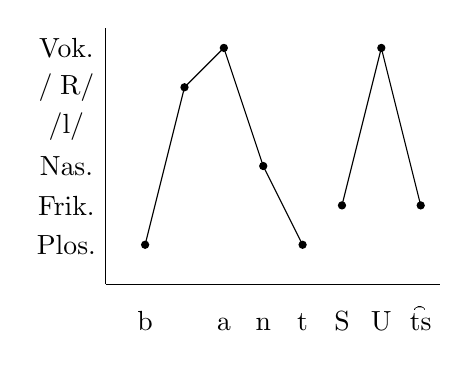
\begin{tikzpicture}[scale=0.5]
\draw[black] (-1,0) -- (7.5,0) ; % x axis
\draw[black] (-1,0) -- (-1,6.5); % y axis
\node at (-2,1) {Plos.};
\node at (-2,2) {Frik.};
\node at (-2,3) {Nas.};
\node at (-2,4) {\textipa{/l/}};
\node at (-2,5) {\textipa{/\;R/}};
\node at (-2,6) {Vok.};
\draw[black] (0,1) -- (1,5) -- (2,6) -- (3,3) -- (4,1);
\draw[black] (5,2) -- (6,6) -- (7,2);
\node at (0,-1) {\strut \textipa{b}};
\node at (1,-1) {\strut \textipa{\textscr}};
\node at (2,-1) {\strut \textipa{a}};
\node at (3,-1) {\strut \textipa{n}};
\node at (4,-1) {\strut \textipa{t}};
\node at (5,-1) {\strut \textipa{S}};
\node at (6,-1) {\strut \textipa{U}};
\node at (7,-1) {\strut \textipa{\t{ts}}};
\fill (0,1) circle [radius=3pt];
\fill (1,5) circle [radius=3pt];
\fill (2,6) circle [radius=3pt];
\fill (3,3) circle [radius=3pt];
\fill (4,1) circle [radius=3pt];
\fill (5,2) circle [radius=3pt];
\fill (6,6) circle [radius=3pt];
\fill (7,2) circle [radius=3pt];
\end{tikzpicture}}
\end{figure}
\end{minipage}
\pause
\begin{minipage}{.05\textwidth}
\hfill
\end{minipage}
\begin{minipage}{.6\textwidth}
\begin{figure}
\centering
\scalebox{.75}{
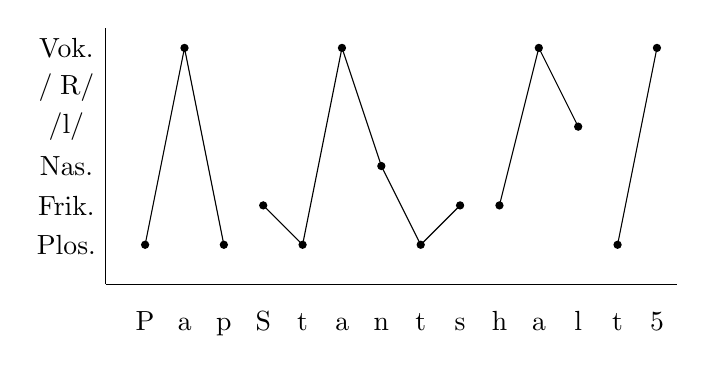
\begin{tikzpicture}[scale=0.5]
\draw[black] (-1,0) -- (13.5,0) ; % x axis
\draw[black] (-1,0) -- (-1,6.5); % y axis
\node at (-2,1) {Plos.};
\node at (-2,2) {Frik.};
\node at (-2,3) {Nas.};
\node at (-2,4) {\textipa{/l/}};
\node at (-2,5) {\textipa{/\;R/}};
\node at (-2,6) {Vok.};
\draw[black] (0,1)--(1,6)--(2,1);
\draw[black](3,2)--(4,1)--(5,6)--(6,3)--(7,1)--(8,2);
\draw[black](9,2)--(10,6)--(11,4);
\draw[black](12,1)--(13,6);
\fill (0,1) circle [radius=3pt];
\fill (1,6) circle [radius=3pt];
\fill (2,1) circle [radius=3pt];
\fill (3,2) circle [radius=3pt];
\fill (4,1) circle [radius=3pt];
\fill (5,6) circle [radius=3pt];
\fill (6,3) circle [radius=3pt];
\fill (7,1) circle [radius=3pt];
\fill (8,2) circle [radius=3pt];
\fill (9,2) circle [radius=3pt];
\fill (10,6) circle [radius=3pt];
\fill (11,4) circle [radius=3pt];
\fill (12,1) circle [radius=3pt];
\fill (13,6) circle [radius=3pt];
\node at (0,-1){\strut \textipa{P}};
\node at (1,-1){\strut \textipa{a}};
\node at (2,-1){\strut \textipa{p}};
\node at (3,-1){\strut \textipa{S}};
\node at (4,-1){\strut \textipa{t}};
\node at (5,-1){\strut \textipa{a}};
\node at (6,-1){\strut \textipa{n}};
\node at (7,-1){\strut \textipa{t}};
\node at (8,-1){\strut \textipa{s}};
\node at (9,-1){\strut \textipa{h}};
\node at (10,-1){\strut \textipa{a}};
\node at (11,-1){\strut \textipa{l}};
\node at (12,-1){\strut \textipa{t}};
\node at (13,-1){\strut \textipa{5}};
\end{tikzpicture}}
\end{figure}
\end{minipage}


\end{frame}
